The focus of this report was cluster finding by unsupervised learning, which gave some workable results. The found clusters can be used to identify behaviour using machine learning techniques. We will give an example of how this can be done in a way that is easy to extend. We will use the clusters that we manually labeled and attach a set of features to them (a set of properties that describe it). With the cluster labels and their features we train a learning algorithm and test its accuracy.

 \subsection{Features}
 The features we came up with consist of numeric values and can be derrived from the cluster data. Some are used for manual annotation and some are values that we hope the learning algorithm can use to find hidden relations. Here is a list with their descriptions:

 \begin{description}
  \item[Duration] The duration of the cluster in seconds.
  \item[Average speed] Average speed during the cluster in km/h.
  \item[Height difference] An estimation of the height traveled in meters. The height is very unreliable, even after removing outliers, so we can not just use the sum of the values. Instead we calculate the derivative of the height numerical (the verticale speed) and take the average value. To make this value more intuitive we multiply it by the duration of the cluster, which results in the average vertical distance traveled.
  \item[Ground distance] Distance between cluster begin- and endpoint in km. 
  \item[Total distance] Total distance traveled in km.
  \item[Angle variance] The average change of direction in degrees per minute. On low resolution it can look like the bird is flying in a straight line, while he is really making sharp turns. Figure \ref{fig:anglevar1} shows a bird\footnote{bird 344, session 10} who seems to be flying straight on his trajectory, while his speeds indicate he is not. For this reason we do not use the angle between two data points, but the angle between two \emph{instantaneous speed vectors}. These are 3d vectors indicating the motion of the bird measured on a small time interval.

\begin{figure}[htb!]
\begin{center}
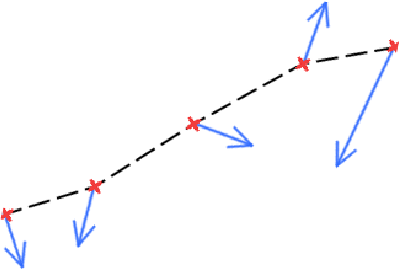
\includegraphics[scale=0.8]{anglevar2.png}
\end{center}
\caption{Trajectory of a bird with his instantaneous speeds} 
\label{fig:anglevar1}
\end{figure}

  There are some problems with this feature, because the instantaneous speed is unreliable. When the resolution is high the time passed between two points is very low, but the angle between them can be a bit jumpy. This results in large changes in angle while the bird is flying straight. We try to limit this error by sampling the data when the resolution is too high (above 1 dat/min is the limit used in our code).
  \item[Distance difference] The difference between \emph{ground distance} and \emph{total distance}. When the bird is hunting he often flies in circles and returns near his startpoint, which is easy to read in this variable (we include this because the learning algorithm can not see spatial information in the trajectory).
  \item[Resolution] The average amount of data points per minute in the clusters data. Not very useful for us but maybe for the learning algorithm.
  \item[Fourier frequencies] Maximum frequency in the fourier transform in the $x$, $y$ and $z$ directions (three features), as explained in TODO. Our fourier transform only returns the frequencies of one point. We currently use the center point for this feature, which is not te best method because that point could contain noise. This can be improved by taking the average of the frequencies of all accelerometer data in the cluster.
  \item[Previous cluster] The id of the previous cluster. This may be needed to recognize some behaviour, like digesting (after hunting).
 \end{description}

 We store the features in a Matlab array and save them to a csv file.

\subsection{Adding Features}
The GPS and accelerometer data can be used to create different features not mentioned above. We did not have the resources to do research in finding the best features, but we wanted to be able to add new ones without re-annotating the data. All features are calculated in \verb|createClusterFeatures.m| and are then saved along with their annotation. When a new feature is thought up it can be appended to the return value of that function. Then \verb|raloadFeatures.m| can be used to recreate the features, transferring all previous annotations. 

 \subsection{Results}
 We then appended all the csv files into a large database of training data. We removed \emph{unknown} and \emph{bad} labeled clusters as they indicate bad clustering or insufficient knowledge of birds. To improve the result we also combined \emph{digesting} and \emph{sleeping} clusters into one class. They can be seperated in future experiments, but with our current features and annotations an algorithm will not find a difference. The training data can then be loaded into a machine learning program. We chose for WEKA\footnote{http://www.cs.waikato.ac.nz/ml/weka/} because it is easy to use and it supports many learning algorithms.

 For the tests we use following dataset:
\begin{itemize}
\item 1637 annotated clusters
\item 12 features
\item 3 classes (Flying, Floating and Diving)
\end{itemize}


WEKA gave the following results, using 10-fold crossvalidation for testing:

\begin{center}
\begin{tabular}{r|c}
	\textnormal{Method} & \textnormal{Precision} \\ \hline 
	Tree J48 & 81\% \\
	Logistic & 82\% \\
	Perceptron & 82\% \\
\end{tabular}
\end{center}


The learning methods yield very similar results. Figure \ref{fig:wekatree} shows the J48 tree that was generated. 
\begin{figure}[htb!]
\begin{center}
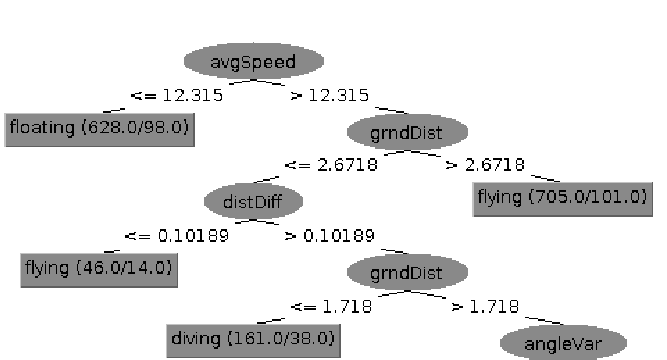
\includegraphics[scale=0.75]{tree2}
\end{center}
\caption{Large part of the WEKA generated tree}
\label{fig:wekatree}
\end{figure}

Most of the errors were made in classifying \emph{diving}, the cunfusion matrix shows this:
\begin{verbatim}
=== Confusion Matrix ===

   a   b   c   <-- classified as
 519  26  22 |   a = floating
  35 632  77 |   b = flying
  64  99 163 |   c = diving
\end{verbatim}
The following table shows the prediction accuracy for each class:
\begin{center}
\begin{tabular}{l|l}
	\textnormal{Class} & \textnormal{Correctly classified} \\ \hline 
	Floating & 91.5\% \\
	Flying &  85.1\% \\
	Diving & 50.0\% \\
\end{tabular}
\end{center}

The data was annotated by 4 different people with very little knowledge of birds, which is probably an other reason for the misclassifications. 
